%& C:\Users\RANGAR~1\AppData\Roaming\TikzEdt\TikzEdt\023~1.0\TEMP_H~1
\begin{document}
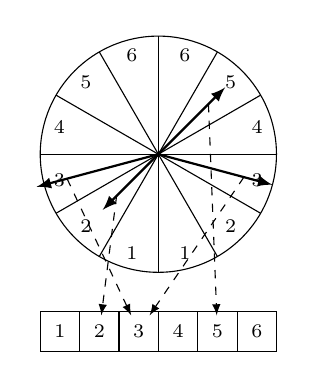
\begin{tikzpicture}[x=1cm, y=1cm, every node/.append style={text=black, font=\scriptsize}]
\def\r{1.5}
	\draw (0,0) coordinate (o) circle (\r);
	\foreach \theta in {-90, -60, ..., 240}
	{
		\draw (o) -- (\theta:\r);
	}
	\foreach \theta/\l in {-60/1, -30/2, 0/3, 30/4, 60/5, 90/6}
	{
		\node at  (\theta - 15:1.3) {$\l$};
	}	
	\foreach \theta/\l in {-90/1, -120/2, -150/3, -180/4, -210/5, -240/6}
	{
		\node at  (\theta - 15:1.3) {$\l$};
	}		
	
	\foreach \theta/\r/\t in {-15/1.5/1, 45/1.2/2, -135/1/3, -165/1.6/4}
	{
		\draw[-latex, thick] (o) -- (\theta:\r ) coordinate [near end] (t\t);
	}
	
	\foreach \i/\l in {-1.25/1, -0.75/2, -0.25/3, 0.25/4, 0.75/5, 1.25/6 }
	{
		\draw (\i-0.25, -2) rectangle ++(0.5, -0.5);
		\node (a\l) at (\i, -2.25) {$\l$} ;
	}
	
	\draw[-latex, dashed] (t1) -- (a3);
	\draw[-latex, dashed]  (t2) -- (a5);
	\draw[-latex, dashed]  (t3) -- (a2);
	\draw[-latex, dashed]  (t4) -- (a3);
	
	

\usetikzlibrary{calc}
\pgftransformreset
\node[inner sep=0pt,outer sep=0pt,minimum size=0pt,line width=0pt,text width=0pt,text height=0pt] at (current bounding box) {};
%add border to avoid cropping by pdflibnet
\foreach \border in {0.1}
  \useasboundingbox (current bounding box.south west)+(-\border,-\border) rectangle (current bounding box.north east)+(\border,\border);
\newwrite\metadatafile
\immediate\openout\metadatafile=\jobname_BB.txt
\path
  let
    \p1=(current bounding box.south west),
    \p2=(current bounding box.north east)
  in
  node[inner sep=0pt,outer sep=0pt,minimum size=0pt,line width=0pt,text width=0pt,text height=0pt,draw=white] at (current bounding box) {
\immediate\write\metadatafile{\p1,\p2}
};
\immediate\closeout\metadatafile
\end{tikzpicture} 

\end{document}
